\chapter{Latent Dirichlet Allocation}

 \begin{figure*}
 \centering
 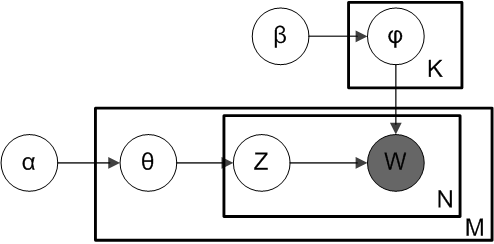
\includegraphics[width=0.5\textwidth]{lda-plate}
 \caption{LDA Plate Notation}
 \label{fig:lda-plate}
\end{figure*}

Latent Dirichlet Allocation (LDA) is a probabilistic generative model which automatically and jointly clusters words into topics and documents into mixture of topics. LDA assumes that documents are a mixture of topics which give out words with certain probabilities. Fig. \ref{fig:lda-plate} represents the plate notation of LDA. The generative process is defined below:
\begin{enumerate}
\item Decide on the total number of words that a document will have, lets say $N$ and there are $M$ no. of documents.
\item Choose $\theta_i \, \sim \, \mathrm{Dir}(\alpha)$ , where $i$ $\in$ $\{ 1,\dots,M \}$ and $\mathrm{Dir}(\alpha)$  is the Dirichlet distribution for parameter $\alpha$.
\item Choose $\phi_k \, \sim \, \mathrm{Dir}(\beta)$ , where  $k \in \{ 1,\dots,K \}$ .
\item For each of the word positions $i, j,$ where  $j \in \{ 1,\dots,N_i \}$ , and  $i \in \{ 1,\dots,M \} $.
\begin{itemize}
\item Choose a topic $z_{i,j} \,\sim\, \mathrm{Multinomial}(\theta_i)$. 
\item Choose a word $w_{i,j} \,\sim\, \mathrm{Multinomial}( \phi_{z_{i,j}})$.
\end{itemize}
\end{enumerate}

